\documentclass[11pt]{article}
\usepackage[utf8]{inputenc} % Para caracteres en espa�ol
\usepackage{amsmath,amsthm,amsfonts,amssymb,amscd}
\usepackage{multirow,booktabs}
\usepackage[table]{xcolor}
\usepackage{fullpage}
\usepackage{lastpage}
\usepackage{enumitem}
\usepackage{floatrow}
\usepackage{multicol}
\usepackage{fancyhdr}
\usepackage{mathrsfs}
\usepackage{wrapfig}
\usepackage[final]{pdfpages}
\usepackage{setspace}
\usepackage{esvect}
\usepackage{calc}
\usepackage{multicol}
\usepackage{cancel}
\usepackage{graphicx}
\graphicspath{ {picturesB/} }
\usepackage[retainorgcmds]{IEEEtrantools}
\usepackage[margin=3cm]{geometry}
\usepackage{amsmath}
\newlength{\tabcont}
\setlength{\parindent}{0.0in}
\setlength{\parskip}{0.05in}
\usepackage{empheq}
\usepackage{framed}
%\usepackage{newtxmath}
\usepackage{euscript}
\DeclareMathAlphabet{\mathpzc}{T1}{pzc}{m}{it}
\usepackage[most]{tcolorbox}
\usepackage{xcolor}
\colorlet{shadecolor}{orange!15}
\parindent 0in
\parskip 12pt
\geometry{margin=1in, headsep=0.25in}
\theoremstyle{definition}
\newtheorem{defn}{Definition}
\newtheorem{reg}{Rule}
\newtheorem{exer}{Exercise}
\newtheorem{note}{Note}
\newcommand{\volume}{{\ooalign{\hfil$V$\hfil\cr\kern0.08em--\hfil\cr}}}
\newcommand{\parr}{\mathbin{\|}} % Parralel Symbol
\begin{document}
\setcounter{section}{1}%Section we want -1
\setcounter{page}{24} %Page we want
\setcounter{equation}{35}%Equation we want -1
\def\thepart{\arabic{part}}
\setcounter{part}{9}
\numberwithin{equation}{part}

 \pagestyle{fancy}
\fancyhf{}
\rhead{Section 9:  Electrostatic Propulsion - Hall-Effect Thrusters}
\rfoot{Page \thepage}
\thispagestyle{empty}

\begin{center}
{\LARGE \bf Section 9:  Electrostatic Propulsion}\\
{\large AE435}\\
Spring 2018
\end{center}
\vspace{5mm}
\section{Hall-Effect Thrusters}
\vspace{25mm}
\tableofcontents
\newpage
Hall thrusters have a cylindrical channel with an interior anode, a magnetic circuit that produces a primarily radial magnetic field across the channel, and a cathode external to the channel.   The details of the channel structure and magnetic field shape determine the performance, efficiency, and lifetime. Anode efficiency 50-60$\%$, specific impulse is around 1000-2000sec but at lower specific impulse has higher thrust at the same power. 

Efficiency and specific impulse are typically lower than ion thrusters, the thrust-to-power ratio is higher and Hall thruster requires fewer power supplies to operate.
 
There are two main types of Hall thrusters:
\begin{enumerate}
\item Hall-effect thruster (HET, a.k.a., Hall thruster, stationary plasma thruster (SPT), magnetic layer thruster are all the same thing)  These devices have a dielectric insulating wall in the plasma channel.  It is typically boron nitride (ceramic insulator).  Ideal because of its low sputtering yield and relatively low secondary electron emission coefficient.
\item Thruster with anode layer (TAL)  Dielectric channel wall is replaced with metallic conducting wall.  Considerably shorter geometry, with strong electric field close to the anode. 
 \end{enumerate}

 \begin{center}
{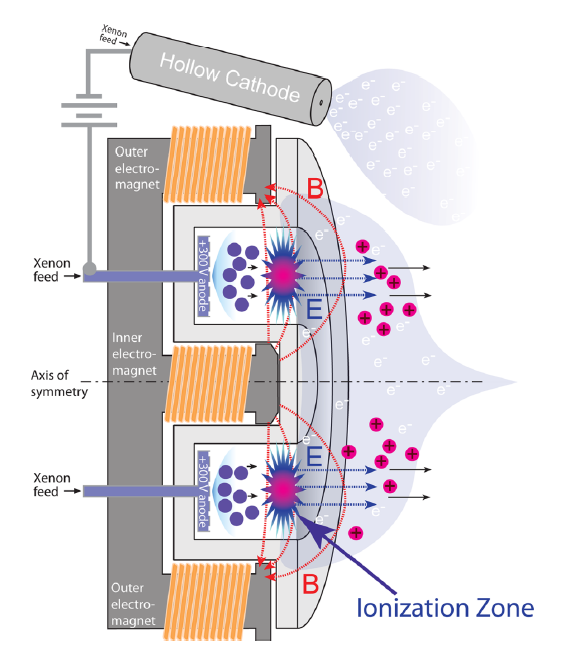
\includegraphics[scale=0.55]{15.png}}
\end{center}

HET is dominant in U.S.  TAL was developed by Russians in 1960s, not as much research focus anymore.  HET tends to have better efficiency and performance due to longer channel for increased ionization path length and lower electron transport.
\begin{center}
{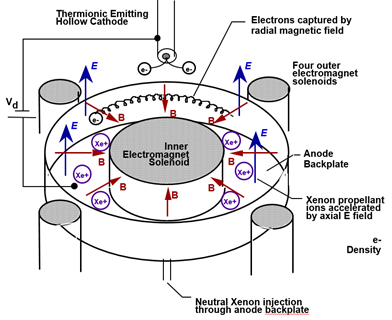
\includegraphics[scale=1.6]{16.png}}
\end{center}
 \begin{center}
{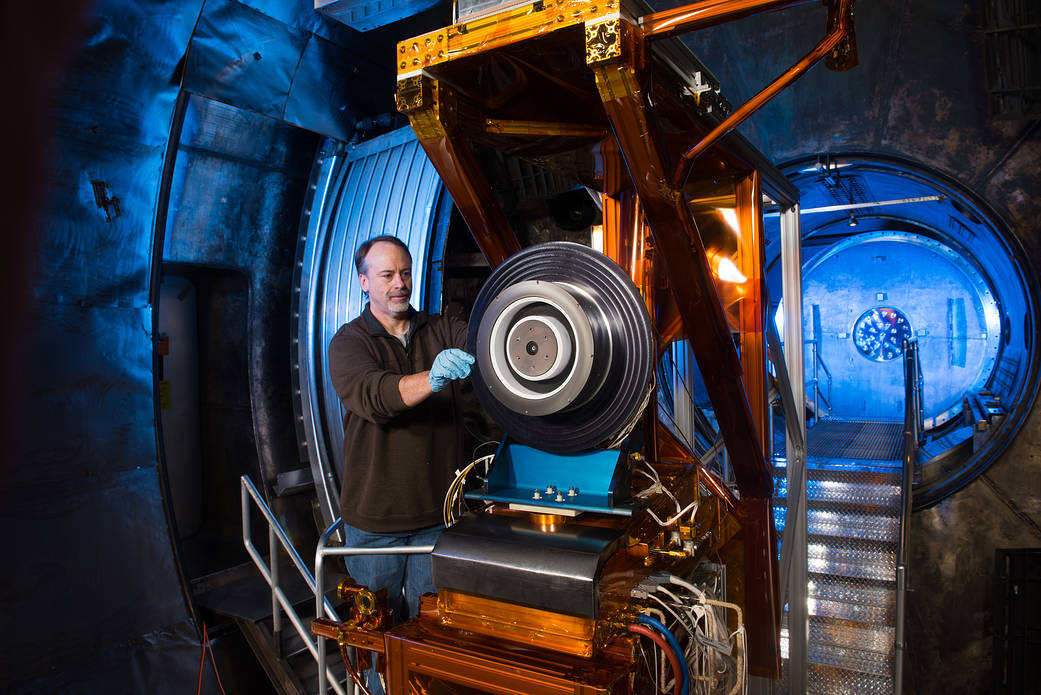
\includegraphics[scale=1.5]{17.jpg}}
\end{center}
12.5kW HERMeS Hall thruster
 \begin{center}
{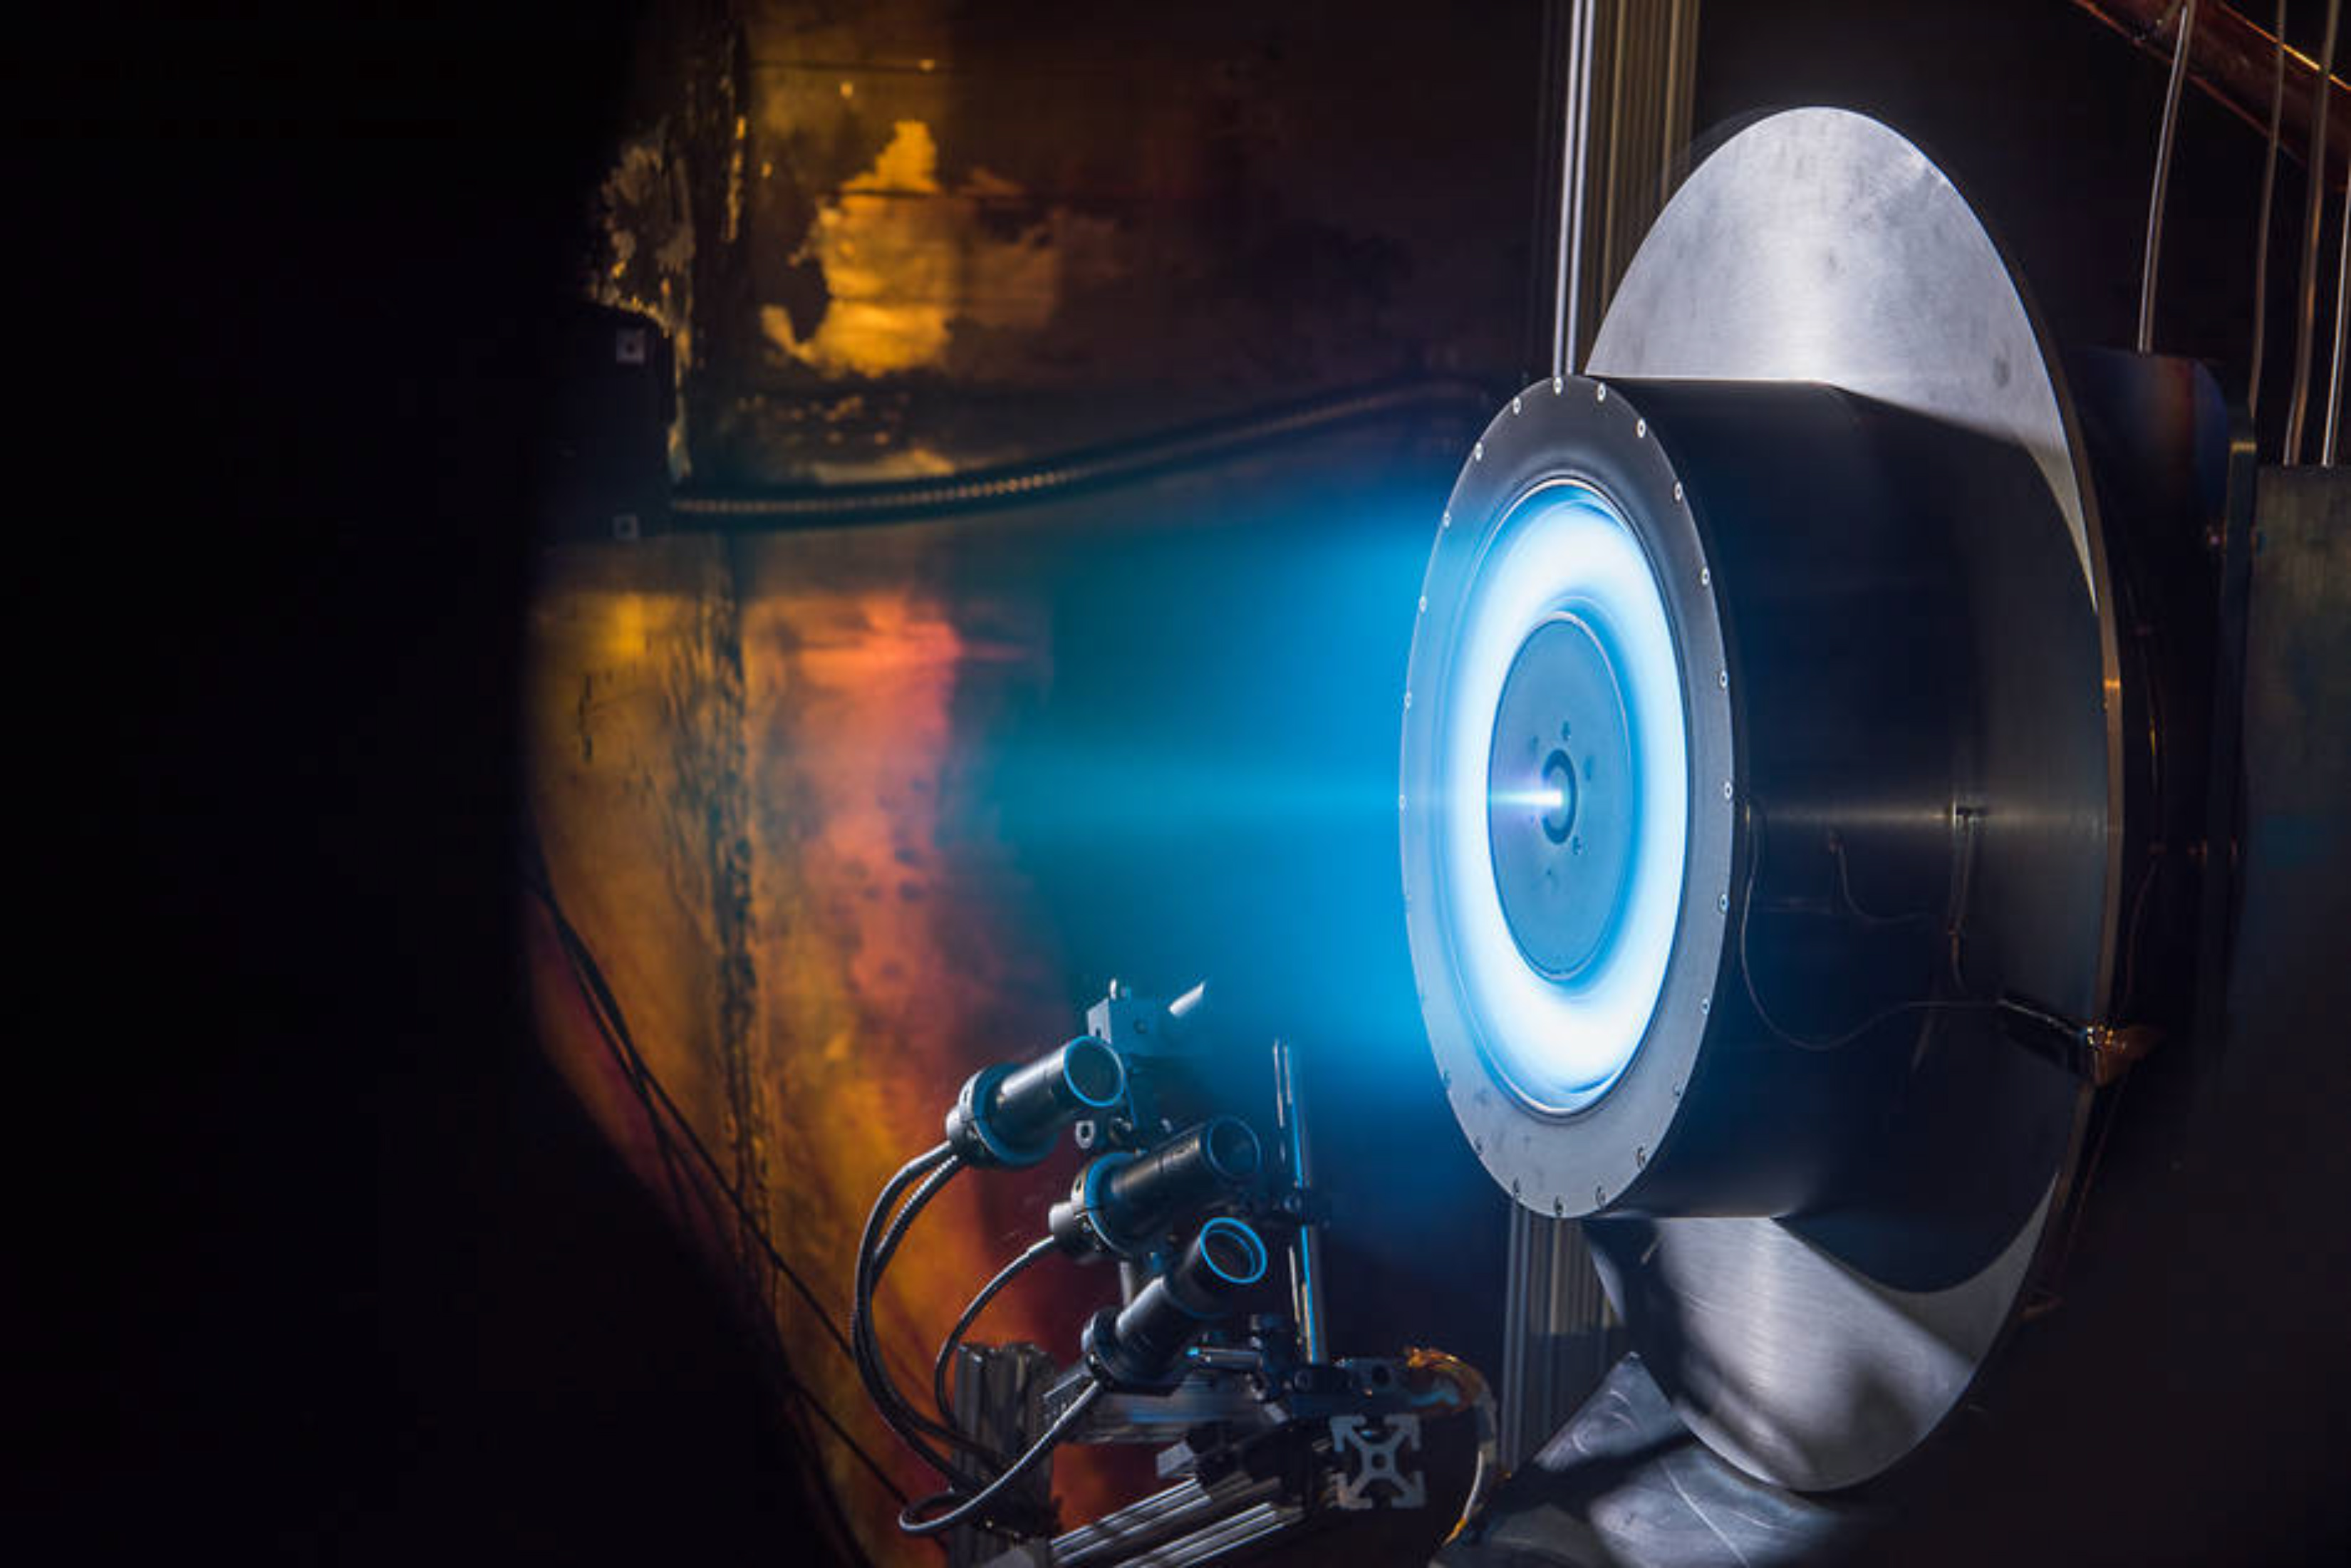
\includegraphics[scale=0.5]{18.jpg}}
\end{center}
 \newpage
PPS-1350 SNECMA
 \begin{center}
{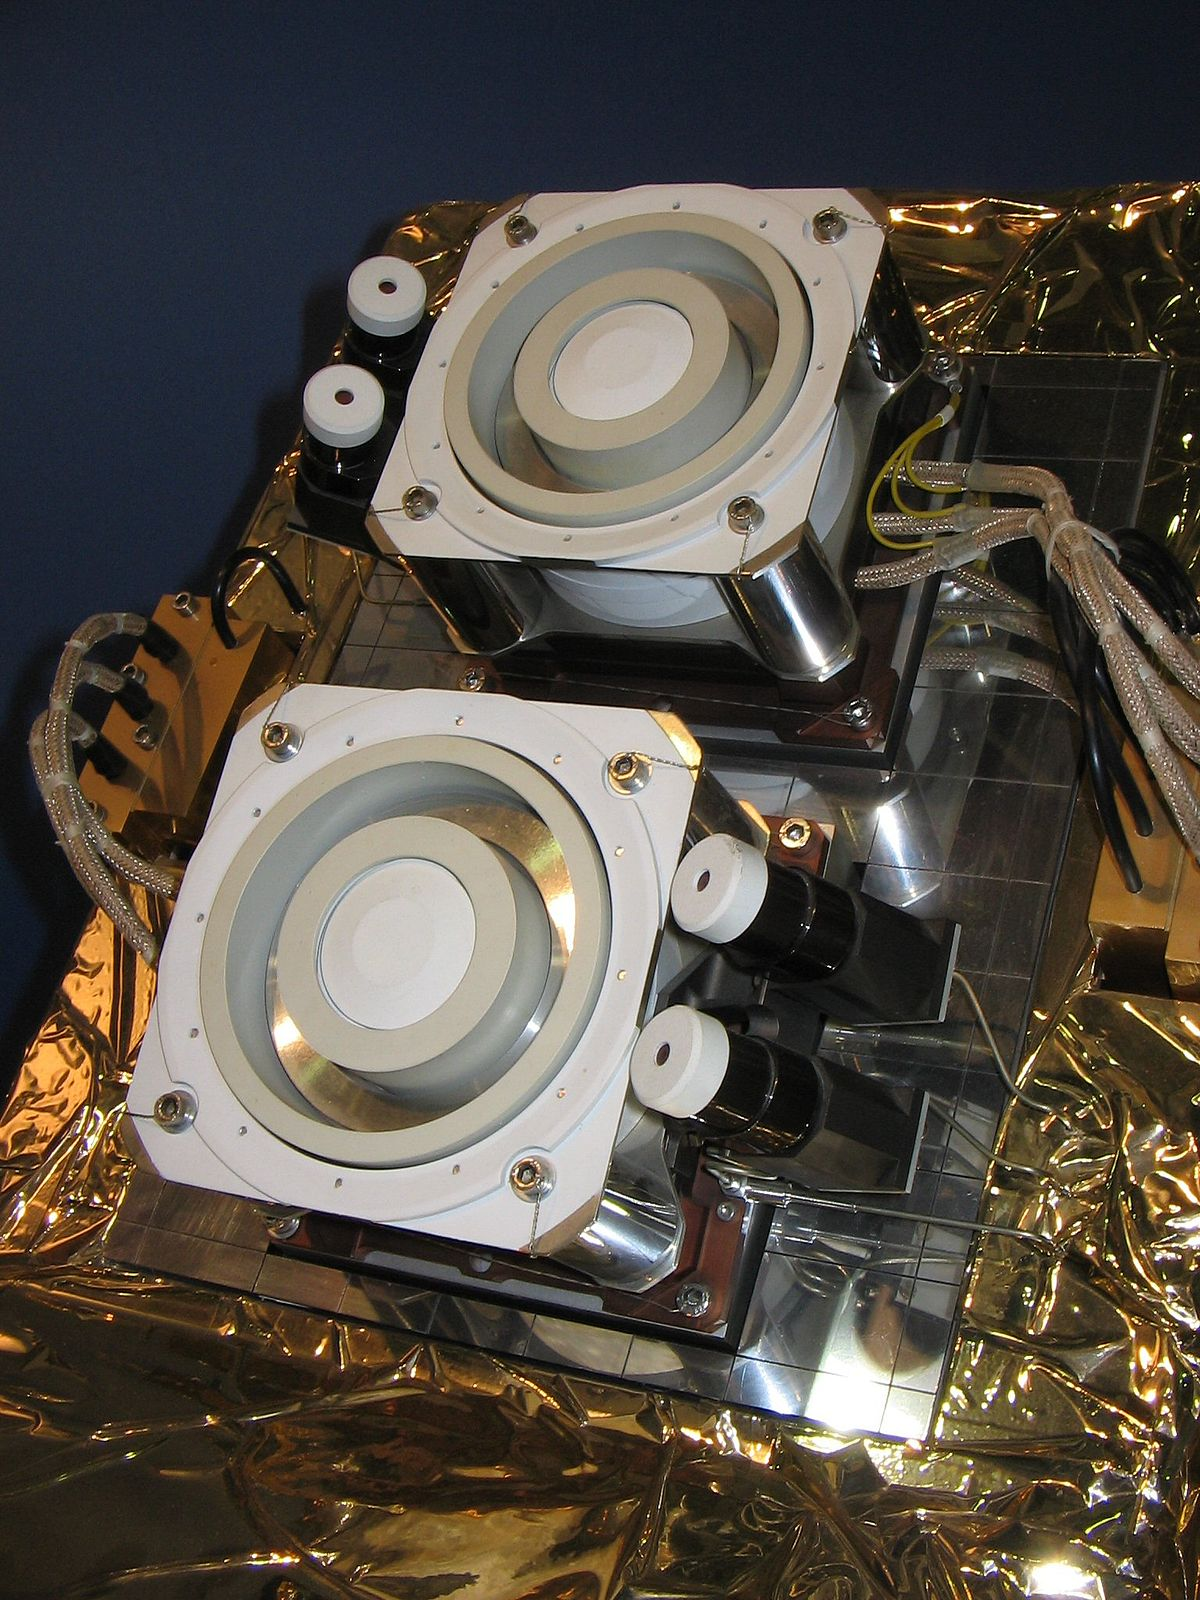
\includegraphics[scale=0.5]{19.jpg}}
\end{center}
 
Aerojet XR-5
\begin{center}
{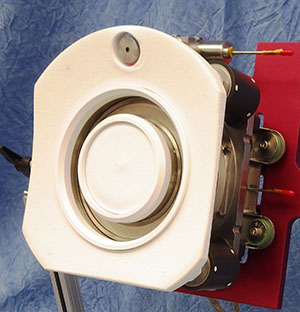
\includegraphics[scale=0.5]{20.jpg}}
\end{center}

 \newpage
\subsection{Operation and Scaling}
Propellant injected at the anode expands toward the exit plane and encounters the plasma generated in the channel.  This crossed field discharge extends over a length scale, L, and produces a significant plasma density of characteristic width, w, which is basically the channel width.  This plasma region is symmetric about the cylindrical channel and has a symmetric area $A_e$.  Applied magnetic field is primarily vertical (radial) in this intense plasma region.%
 
 %Magnetic field is having a significant effect on thier motion.
In Hall thruster the electrons are magnetized and forced to execute ExB drift in the azimuthal direction.  Therefore we require the electron Larmor radius to be much smaller than the characteristic size of the plasma length scale, L, that is:
 \begin{equation}
 \begin{aligned}
 r_{L,e} = \frac{V_{th}}{\omega_B} = \frac{m}{e \, B} \sqrt{\frac{8 \, k \, T_e}{\pi \, m}} \ll L
 \end{aligned}
 \end{equation}
 
And the electron Hall parameter must be much greater than 1.
 
  \begin{equation}
 \begin{aligned}
 \Omega_e^2 = \frac{\omega_B^2}{\nu^2} \gg 1
 \end{aligned}
 \end{equation}
 Where
   \begin{equation*}
 \begin{aligned}
\nu &=\text{Total collision frequency of electrons}\\
\omega_B &=\text{Cyclotron frequency of electrons}
 \end{aligned}
 \end{equation*}
 


We saw that a large value of the Hall parameter reduces the cross-field electron mobility in (III. B. 2.).
 
Similarly, we require the ions to NOT be magnetized, that is, the ion Larmor radius is much larger than the characteristic size, L. We want the ions to just shoot straight out so we don't want them experience an ExB drift.
 
  \begin{equation}
 \begin{aligned}
  r_{L,i} = \frac{V_{i}}{\omega_B} = \frac{M}{e \, B} \sqrt{\frac{2 \,e \, V_b}{M}} \gg L
 \end{aligned}
 \end{equation}
 
where beam voltage, $V_b$, the total potential drop that is accelerating the ions.
 \newpage
The magnetic field have a typical axial profile as shown below.  $dB/dz > 0$ critical for stability!
\begin{center}
{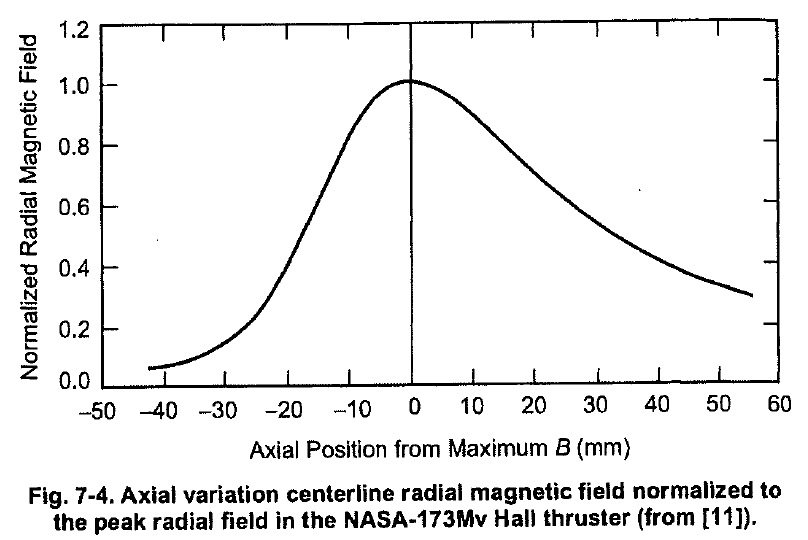
\includegraphics[scale=0.65]{21.png}}
\end{center}
\begin{center}
{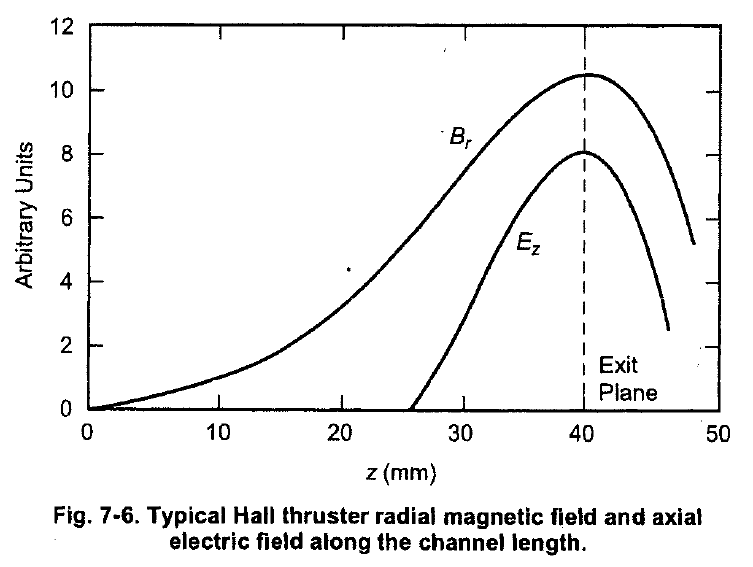
\includegraphics[scale=0.65]{22.png}}
\end{center}
Notice dB/dz is greater than 1 so the 0 location is the exit plane, everything to the left is inside the discharge chamber, and everything to the right is outside the discharge chamber. 
 
What if we had a negative dB/dz? We would have another trapping region within the channel which is not desired.
 
The region of high magnetic field is at the exit plane (peak field ~150-200 G), and is where the electrons are confined and therefore where the largest potential drop occurs (and therefore largest electric field, ).  Ions are accelerated by this electric field and this region is called the "acceleration region".  The "ionization" region precedes it, but the two overlap to give rise to a spread in the beam energy (unlike ion thruster which has distinct/separated plasma creation and acceleration regions).


 \subsubsection{Hall Curent Scaling}
\begin{center}
{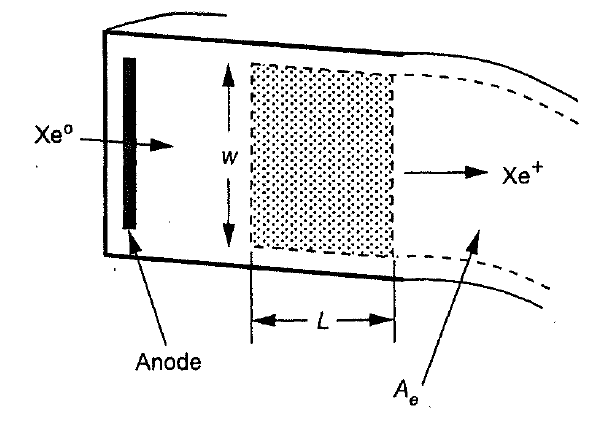
\includegraphics[scale=0.65]{23.png}}
\end{center}
In the strong $B_r$ and $E_z$ region, electrons move in Hall current in azimuthal direction.  That is, they ExB drift, with velocity given by (3.17):
  \begin{equation}
 \begin{aligned}
 |v_{_{E\times B}}| = \frac{E_z}{B_r}
 \end{aligned}
 \end{equation}
 The hall current is then:
 \begin{shaded}
 \textbf{Hall Current:}
  \begin{equation}
 \begin{aligned}
 I_H \cong n_e \, e  \, \omega \, \frac{V_d}{B}
 \end{aligned}
 \end{equation}
where
  \begin{equation*}
 \begin{aligned}
\omega &= \text{Plasma height or channel height}\\
V_d \approx V_b &= \text{Discharge voltage, which is also approximately beam voltage }\\
\end{aligned}
 \end{equation*}
\end{shaded}
\newpage
Hall current is approximately constant for given plasma density or beam current, and is proportional to the discharge voltage.  Since the ion current leaving the plasma to form the beam is:
 
 %Increase the magneitci field, the current decreases. 
 
  \begin{equation}
 \begin{aligned}
 I_i = n_i \, e \, v_i \, A_e \cong n_i \, e \, \sqrt{\frac{2 \, e \, V_d}{M}} \, 2 \, \pi \, R \, \omega
 \end{aligned}
 \end{equation}
where
  \begin{equation*}
 \begin{aligned}
R &= \text{Average Radius of the Plasma Channel} \\
2 \, \pi \, R \, \omega &\sim A_e
 \end{aligned}
 \end{equation*}
 
Then, using (9.41) in (9.40), the hall current becomes:
 
  \begin{equation}
 \begin{aligned}
 I_H \cong \frac{I_i}{2 \, \pi \, R \, B} \, \sqrt{\frac{M \, V_d}{2 \, e}}
 \end{aligned}
 \end{equation}
 
Increasing beam current will increase the circulating Hall current for a given magnetic field and discharge voltage.
We also see increasing magnetic field will decreases the hall current. We will see hall currents range from 10's-100's of Amps. Ion currents are around 1-10's of amps. 
 
\subsubsection{Ionization Length and Scaling}
When we put in the neutrals, we want to ionize all of the nuetrals. We will find a length scale that allows us to have ionization for different characteristics. In other words, neutrals enter the "ionization" region and become ionized.  A flux of neutrals enters the "ionization" region and this flux will decrease with distance into the region as neutrals become ionized.  To ionize most/all of the neutrals, the plasma must have some thickness, L, which we can estimate here. 
 
The rate of change of neutral atoms due to ionization is:
  \begin{equation}
 \begin{aligned}
 \frac{\mathrm{d} n_n}{\mathrm{d} t} = -n_n \, n_e \, <\sigma_i \, v_e>
 \end{aligned}
 \end{equation}%Decreasing with time becuase the amount of neturals to ionize is decreasing as we ionize more and more.
 
where we define the flux as: %Number per second per unit area. 
  \begin{equation}
 \begin{aligned}
 \Gamma_n = n_n \, v_n
 \end{aligned}
 \end{equation}
 
Equation 9.43 then becomes: 
 
  \begin{equation*}
 \begin{aligned}
 \frac{\mathrm{d} \Gamma}{\mathrm{d} t} = \frac{\mathrm{d} n}{\mathrm{d} t}\frac{\mathrm{d} z}{\mathrm{d} t} + n_n \, \frac{\mathrm{d}^2 z}{\mathrm{d} t^2}
 \end{aligned}
 \end{equation*}
 Where
   \begin{equation*}
 \begin{aligned}
\frac{\mathrm{d} z}{\mathrm{d} t} & = v_n & \qquad &\text{Neutral Velocity}\\
n_n \, \frac{\mathrm{d}^2 z}{\mathrm{d} t^2} &= 0 & \qquad &\text{No Neutral Acceleration}
 \end{aligned}
 \end{equation*}
 Such that...
  \begin{equation}
 \begin{aligned}
 \frac{\mathrm{d} \Gamma}{\mathrm{d} t} = \frac{-n_n \, n_e \, <\sigma_i \, v_e>}{n_n \, v_n}\,\mathrm{d}z = \frac{-n_e \, <\sigma_i \, v_e>}{v_n}\,\mathrm{d}z
 \end{aligned}
 \end{equation}
 
which has solution:
  \begin{equation}
 \begin{aligned}
 \Gamma_n(z) = \Gamma(0)\exp(\frac{-z}{\lambda_i})
 \end{aligned}
 \end{equation}
where $\Gamma(0)$ is $\Gamma$ at $z = 0$.

And the ionization mean free path is:
 
  \begin{equation}
 \begin{aligned}
 \lambda_i = \frac{v_n}{n_e <\sigma_i \, v_e>}
 \end{aligned}
 \end{equation}%average distance a neutral particle must travel before it becomes ionized
 
The fraction of neutrals that are ionized after traversing a plasma of length L is:
 %In other words, the flux (ionized neutrals) coming out over the flux (neutrals) coming in
  \begin{equation}
 \begin{aligned}
 \frac{\Gamma_{\text{exit}}}{\Gamma_{\text{incident}}} = 1 - \exp\bigg(\frac{-L}{\lambda_i}\bigg)
 \end{aligned}
 \end{equation}%How the flux changes as the numver of neutrals moves through the plasma.
 
For example, to have 95$\%$ ionized, then the length scale we seek is:
 
  \begin{equation}
 \begin{aligned}
 L = -\lambda_i \, \ln(1-0.95) = 2.996 \, \lambda_i \cong \frac{3 \, v_n}{n_e <\sigma_i \, v_e>}
 \end{aligned}
 \end{equation}
 
or, the plasma thickness $(L)$ must be at least 3 times the ionization mean-free path.  But some ions will hit the channel walls and re-enter the plasma as neutrals, so the plasma thickness, $L$ , should significantly exceed the ionization mean free path, that is:
 
  \begin{equation}
 \begin{aligned}
 \frac{\lambda_i}{L} \ll 1
 \end{aligned}
 \end{equation}
 
Tradeoff: Length-scale long enough to ionize the propellant but not long enough where we deposit a lot of our energy to the channel walls. 
 
Notice in 9.49 how L changes for $v_n$, where $v_n$ is the neutral velocity. Lets say we go from xenon neutrals to krypton or argon neutrals.What happens to $v_n$, they will decrease. Temperature of neutrals coming into chamber are coming through the anode will be around 500Cish, much lower than electron temperature. If the mass of the propellant decreases, the neutral velocity increases , therefor the length scale will need to be longer assuming the same ionization rate. 

Clearly, higher ionization rate leads to a shorter ionization thickness, we don't need it to be that long if we can ionize much quicker. 
 
From our example above, this ratio should be $< 1/3 = 0.33$.
 
Actual channel length is L (plasma thickness), plus the length required to demagnetize the plasma at the anode.  Needs to be long enough so that the Bfield decreases at the anode and particles not magnetized at the anode.  This axial magnetic field gradient of the radial magnetic field is critical for thruster performance, and results in higher thruster efficiency, $\frac{\partial B}{\partial z} > 0$.
 
Want almost zero field at the anode (helps maintain plasma at the anode potential, reduces sheath potential drop), but want strong radial field at exit.  Additionally, magnetic field profile at the thruster exit strongly affects closed electron drifts in azimuthal direction AND has ability to focus ions in axial direction AND can reduce ion bombardment of the walls, improving ion trajectories. 
\begin{center}
 \begin{table}[H]
 \centering
 \begin{tabular}{|c|l|r|r|}
  \hline
 && \\&&\\ &&\\ && \\
 \parbox[t]{2mm}{\multirow{1}{*}{\rotatebox[origin=c]{90}{Standard Model}}} & \hspace{80mm} &  \hspace{70mm} \\&& \\&&\\ && \\&&\\ && \\&&\\&&\\&&\\ && \\
 \hline
  \hline
 && \\&&\\ &&\\ && \\
 \parbox[t]{2mm}{\multirow{1}{*}{\rotatebox[origin=c]{90}{Ion Focusing Bfield}}} & \hspace{80mm} &  \hspace{70mm} \\&& \\&&\\ && \\&&\\ && \\&&\\&&\\&&\\ && \\
 \hline
   \hline
 && \\&&\\ &&\\ && \\&&\\&&\\&&\\
 \parbox[t]{2mm}{\multirow{1}{*}{\rotatebox[origin=c]{90}{Magnetic Shielding}}} & \hspace{80mm} &  \hspace{70mm} \\&& \\&&\\ && \\&&\\ && \\&&\\&&\\&&\\ && \\&&\\&&\\
 \hline
 \end{tabular}
 \end{table}
\end{center}
Additionally, properly designed HET ionizes almost all propellant, such that:
 
Then with (9.42) Hall current:
 
 
Ionization region length must increase with neutral gas velocity, and can decrease with ionization rate coefficient.
 
Additional scaling laws for optimized Hall thrusters are:
 
 
 
 
 
where R is outside radius of the channel.  Optimum current density is essentially constant as the thruster size changes.  Typical current density is 0.1 to 0.15 A/cm2.  At given discharge voltage, power density in a Hall thruster is also constant.  Higher power density requires increasing voltage.
 \begin{center}
{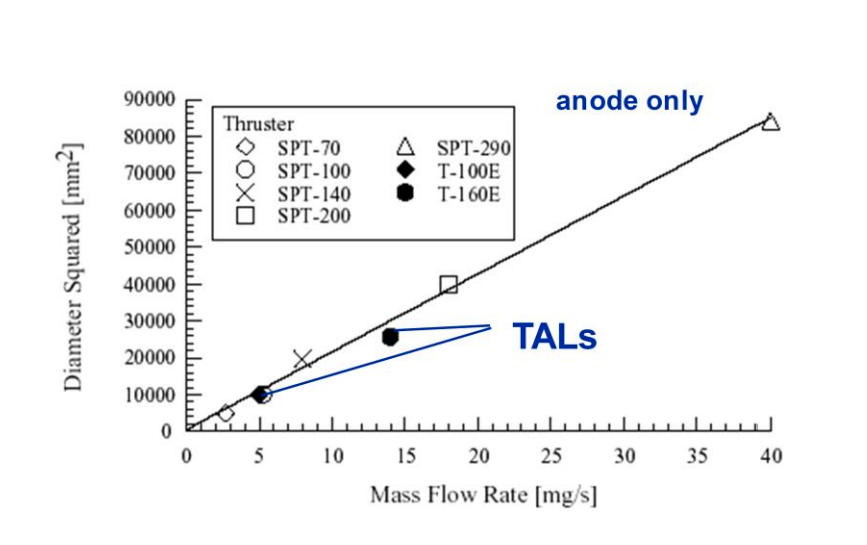
\includegraphics[scale=0.5]{24.png}}
\end{center}
 
\underline{Xenon Rule of 10's}

For xenon, 1 A of thruster current requires approximately 1 mg/s of propellant, which is approximately 10 sccm (standard cubic centimeters per minute) of volumetric flow rate
 
\underline{Magnetic Shielding} 

Recently magnetic shielding has been developed to keep ions from accelerating into and bombarding the channel walls.  Significantly increases lifetime (almost infinite lifetime).
 
 \begin{center}
{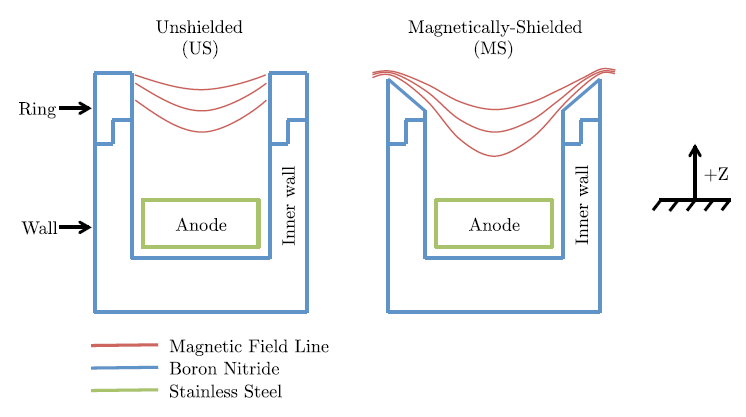
\includegraphics[scale=0.5]{25.png}}
\end{center}
Hofer, Journal Applied Physics, 2014
 


\newpage
\subsection{Electrical Schematic and Current}

Hall thruster electrical schematic:
Heater supply: raise emitter in hollow cathode to thermionic emission temperature
Keeper supply:  ignition and stable cathode operation
Discharge supply:  connected between anode and cathode common (and also thruster body and magnetic circuit)
Magnet supply:  supply current to electromagnets to create magnetic field
 
Once discharge started, cathode heater is turned off and cathode runs in "self-heating" mode.  Keeper used only during start-up, turned off when thruster started.
 
Difference between cathode potential and beam potential is the "coupling voltage".  This is the potential required to extract current from the hollow cathode (typically ~10-20 V, or 5-10% of Vd).  Note the cathode potential will typically be a few volts below space ground (or vac chamber ground in ground tests).
 
The beam voltage is:
 
In lab experiments, the potential between beam and ground is typically small, so:
 
where cathode-to-ground voltage is
 
Average beam ion velocity is then:
 
where average beam voltage is
 
Discharge current is net current through discharge supply, and is the electron and ion current arriving at the anode:
 
 
Discharge current can also be written as the current to the cathode:
 
 
So we see that the discharge current is approximately the electron current emitted by the cathode which is the electron current collected by the anode.
 
 
 
A schematic of the current in the discharge is shown below.
 
Current to the anode is electron current emitted by the cathode, and electron current due to secondary electrons from ionization events.  That is:
 
 
But as we saw in (9.56c), the discharge current is also essentially the electron current emitted by the cathode, that is:
 
 
We recognize that one electron and one ion are made in each ionization event, such that                    	and, therefore (9.57a) becomes,
 
 
This is the net current crossing the exit plane, so discharge current is the ion beam current plus the backstreaming electron current crossing the exit plane.
 
 
Finally, comparing (9.57b) and (9.57c), we see:
 
 
These particles in (9.57d) do not contribute to the discharge current through the discharge supply.  Note in the electrical schematic the entire discharge floats (is not connected to ground).  So there is no return path for these particles to the discharge supply.
 



\end{document}